% --------------------------------------------------------------------------------

\begin{exercise}[Exercise 2.3]

In the comparison shown in Figure \ref{fig:1} (below), with method will perform best in the long run in terms of cumulative reward and probability of selecting the best action?
How much better will it be?
Express your answer quantitatively.

\begin{figure}[H]
    \centering
    \subfloat
    {
        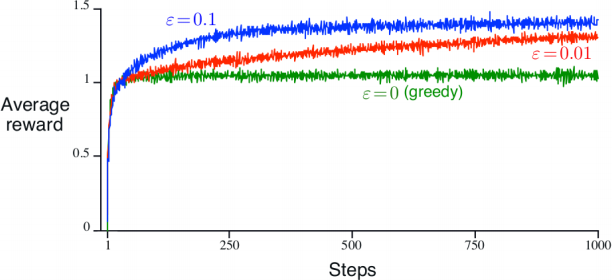
\includegraphics[width = 0.475 \textwidth]{1.3.1.png}
    }
    \subfloat
    {
        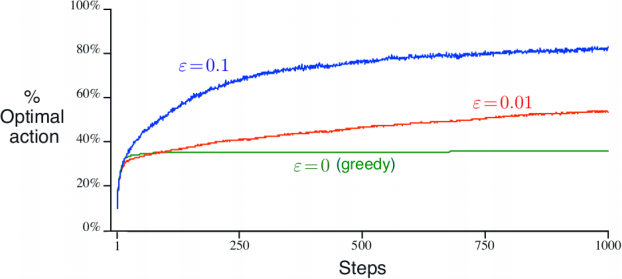
\includegraphics[width = 0.475 \textwidth]{1.3.2.png}
    }
    \hspace{0mm}
    \caption
    {
        Average performance of $\varepsilon$-greedy action-value methods on $10$-armed testbed.
        These data are averages over $2000$ runs with different bandit problems.
        All methods used sample averages as their action-value estimates.
    }
    \label{fig:1}
\end{figure}


\end{exercise}

% --------------------------------------------------------------------------------

\begin{solution}

Obviously, in the long run the $\varepsilon$-greedy methods are no match for the greedy method, since the latter ist likely to get stuck in a local optimum.
Because the $0.1$-greedy method does (on average) $10$ times more exploration than the $0.01$-greedy method, it is a faster learner.
However, once they have both reached a common average expected reward, exploration will no longer be necessary.
Hence, in the long run, the $0.01$-greedy method will likely be $10$ times better than the $0.1$-greedy method.
It is also possible to reduce $\varepsilon$ over time to try to get the best of both high and low values.

\end{solution}

% --------------------------------------------------------------------------------
